\chapter{Exercise 5}
The purpose of the exercise is to understand the principles of 2D
texture mapping and how it can be used for polygon meshes.
Furthermore, the purpose of the exercise is to understand the
process of hidden surface removal and back-face culling.

\section{Part 1}
Hidden surface removal uses z-buffer to update the color of a pixel. Below
we can see two pictures of a scene rendered with and without depth test.

\begin{figure}[ht!]
	\begin{center}
		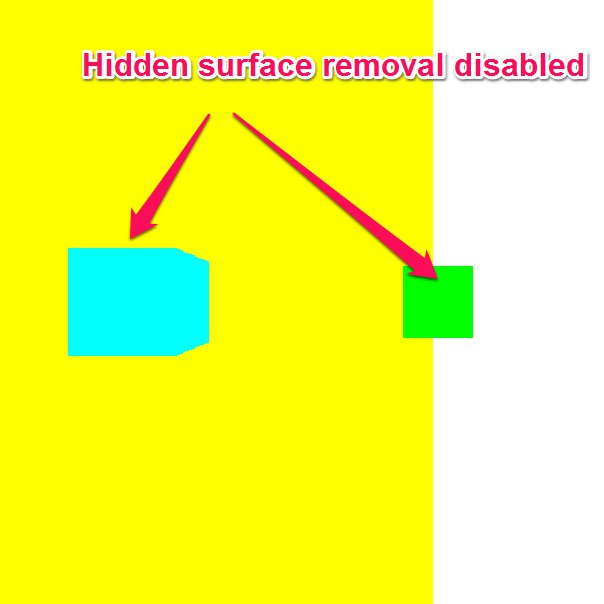
\includegraphics[width=0.28\textwidth]{figures/exercise_6_part_1_1}
	\end{center}
	\vspace{-4.5ex}\caption{Exercise 6 part 1-1 output}
	\label{fig:exercise_6_part_1_1} 
\end{figure}
\begin{figure}[ht!]
	\begin{center}
		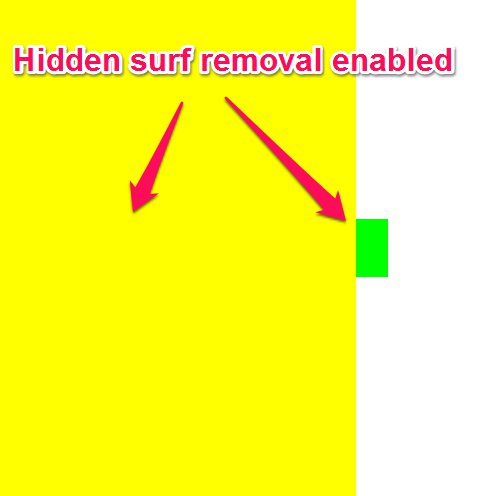
\includegraphics[width=0.28\textwidth]{figures/exercise_6_part_1_2}
	\end{center}
	\vspace{-4.5ex}\caption{Exercise 6 part 1-2 output}
	\label{fig:exercise_6_part_1_2} 
\end{figure}

OpenGL makes use of normal vector to the surface and its angle with camera view direction
to judge if the surface is front or back facing. Below we can see some screenshots
with various culling modes.

\begin{figure}[ht!]
	\begin{center}
		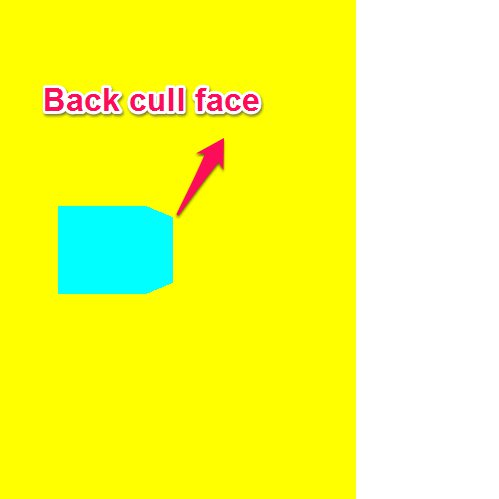
\includegraphics[width=0.3\textwidth]{figures/exercise_6_part_2_1}
	\end{center}
	\vspace{-4.5ex}\caption{Exercise 6 part 2-3 output}
	\label{fig:exercise_6_part_2_1} 
\end{figure}
\begin{figure}[ht!]
	\begin{center}
		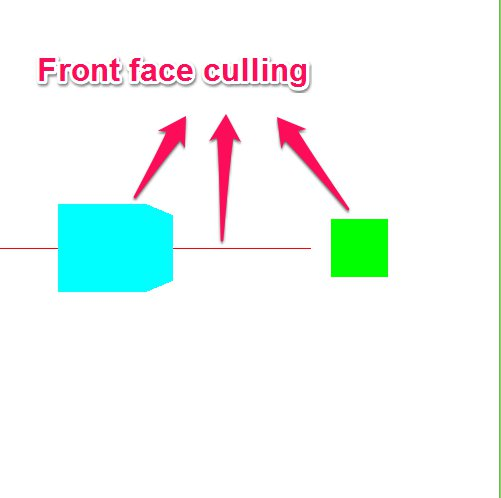
\includegraphics[width=0.3\textwidth]{figures/exercise_6_part_2_2}
	\end{center}
	\vspace{-4.5ex}\caption{Exercise 6 part 1-4 output}
	\label{fig:exercise_6_part_2_2} 
\end{figure}
\begin{figure}[ht!]
	\begin{center}
		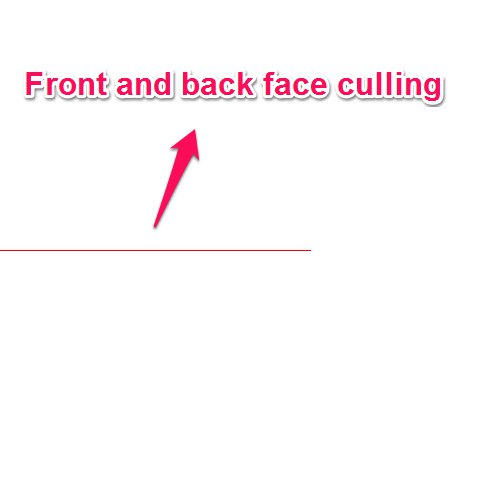
\includegraphics[width=0.3\textwidth]{figures/exercise_6_part_2_3}
	\end{center}
	\vspace{-4.5ex}\caption{Exercise 6 part 1-5 output}
	\label{fig:exercise_6_part_2_3} 
\end{figure}
\clearpage

\section{Part 2}
Using a near frustum value of $9.5$ and far value of $11.0$ with angle of 30 degrees 
I obtained parts of front and back of teapot clipped away. The results are in the figure
\ref{fig:exercise_6_part_3}

\begin{figure}[ht!]
	\begin{center}
		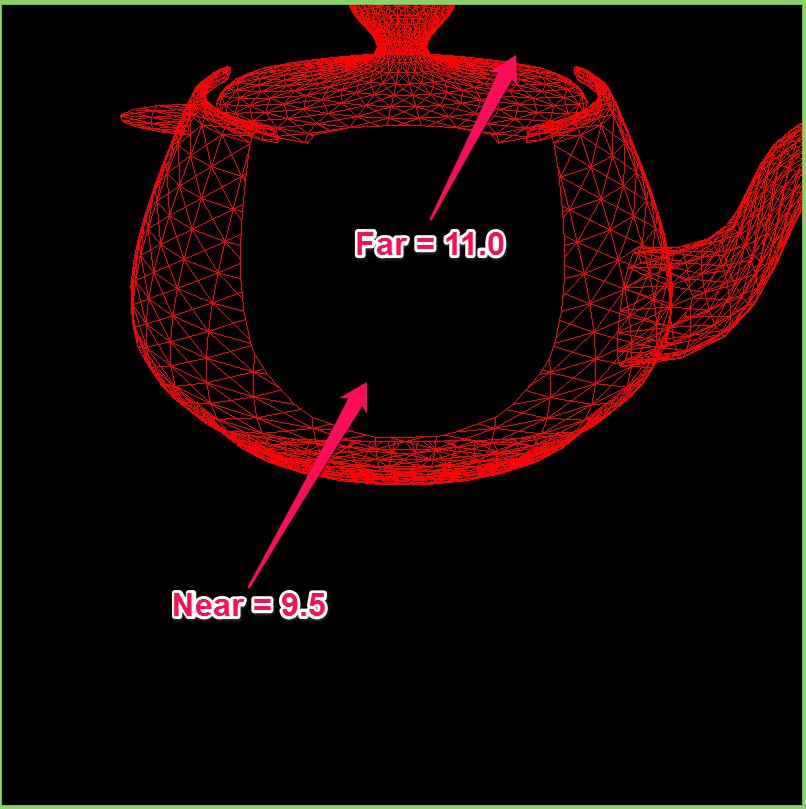
\includegraphics[width=1.0\textwidth]{figures/exercise_6_part_3}
	\end{center}
	\vspace{-4.5ex}\caption{Exercise 6 part 2 output}
	\label{fig:exercise_6_part_3} 
\end{figure}
\clearpage

\section{Part 3}
Using function glTexParameteri I obtained different texture filter techniques as it can
be seen in figures below.

\begin{figure}[ht!]
	\begin{center}
		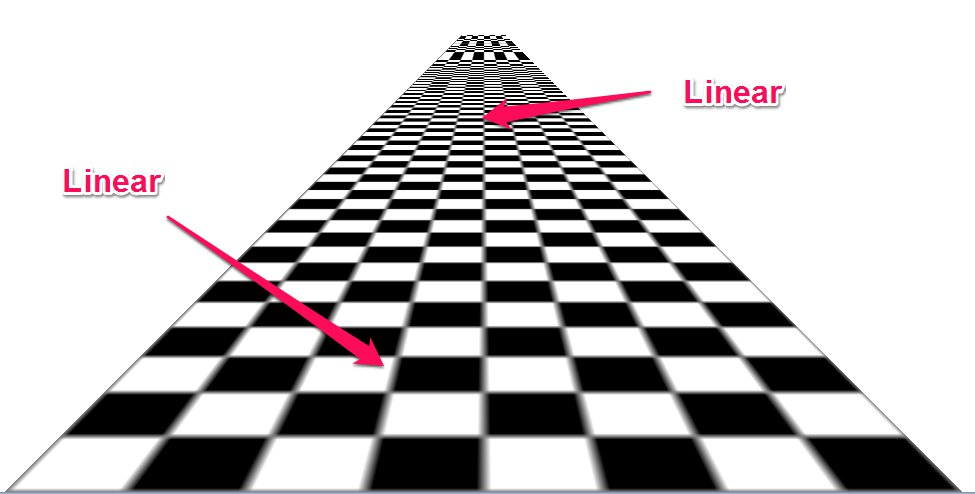
\includegraphics[width=0.45\textwidth]{figures/exercise_6_part_4_1}
	\end{center}
	\vspace{-4.5ex}\caption{Exercise 6 part 3-1 output}
	\label{fig:exercise_6_part_4_1} 
\end{figure}
\begin{figure}[ht!]
	\begin{center}
		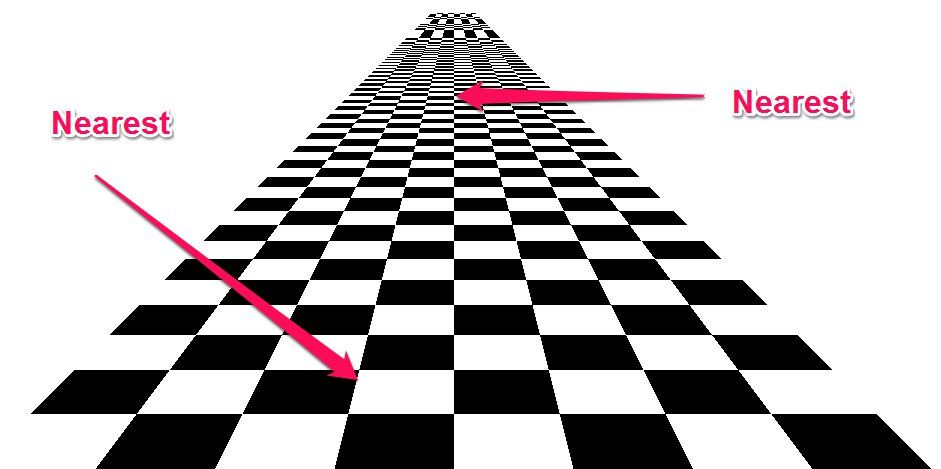
\includegraphics[width=0.45\textwidth]{figures/exercise_6_part_4_2}
	\end{center}
	\vspace{-4.5ex}\caption{Exercise 6 part 3-2 output}
	\label{fig:exercise_6_part_4_2} 
\end{figure}
\begin{figure}[ht!]
	\begin{center}
		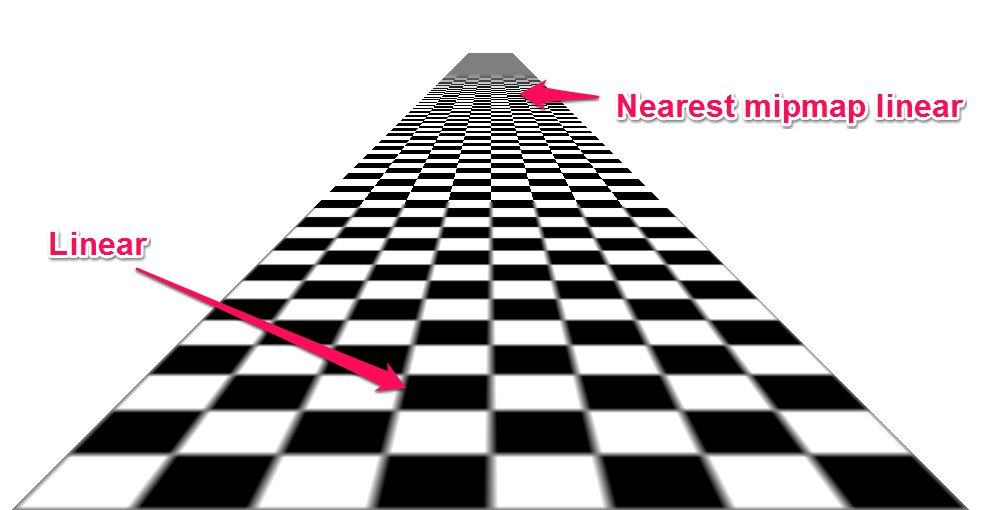
\includegraphics[width=0.45\textwidth]{figures/exercise_6_part_4_3}
	\end{center}
	\vspace{-4.5ex}\caption{Exercise 6 part 3-3 output}
	\label{fig:exercise_6_part_4_3} 
\end{figure}
\begin{figure}[ht!]
	\begin{center}
		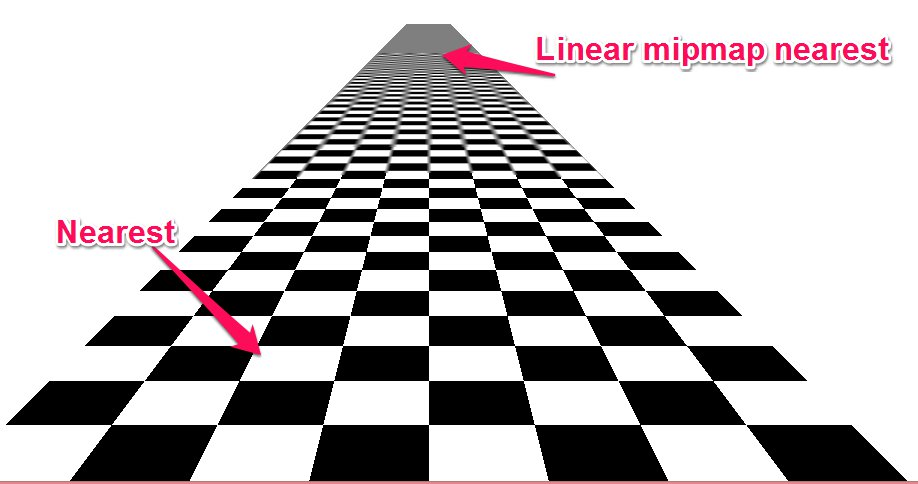
\includegraphics[width=0.45\textwidth]{figures/exercise_6_part_4_4}
	\end{center}
	\vspace{-4.5ex}\caption{Exercise 6 part 3-4 output}
	\label{fig:exercise_6_part_4_4} 
\end{figure}

\section{Part 4}
After modification of polygon and texture vertices I got results shown below for
several configurations of texture wrapping.

\begin{figure}[ht!]
	\begin{center}
		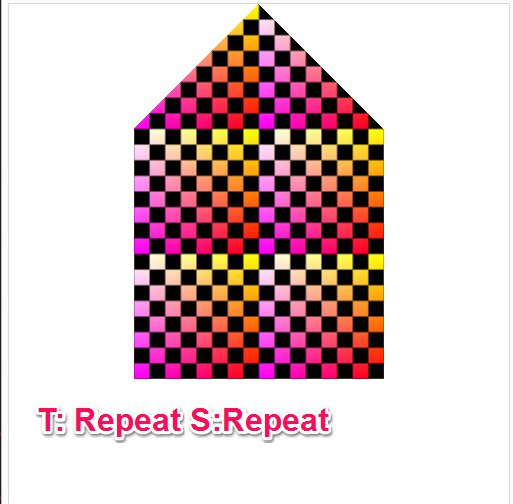
\includegraphics[width=0.35\textwidth]{figures/exercise_6_part_5_1}
	\end{center}
	\vspace{-4.5ex}\caption{Exercise 6 part 4-1 output}
	\label{fig:exercise_6_part_5_1} 
\end{figure}
\begin{figure}[ht!]
	\begin{center}
		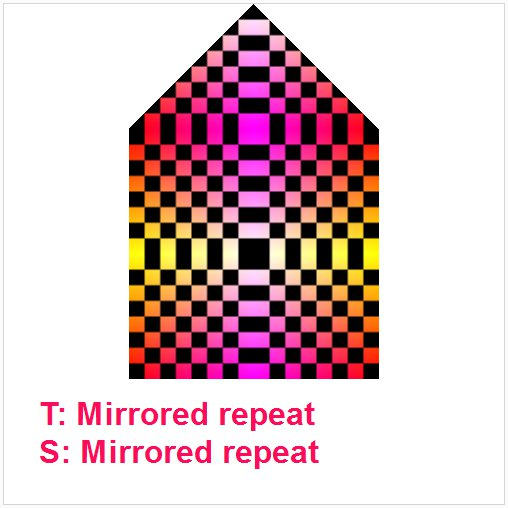
\includegraphics[width=0.35\textwidth]{figures/exercise_6_part_5_2}
	\end{center}
	\vspace{-4.5ex}\caption{Exercise 6 part 4-3 output}
	\label{fig:exercise_6_part_5_3} 
\end{figure}
\begin{figure}[ht!]
	\begin{center}
		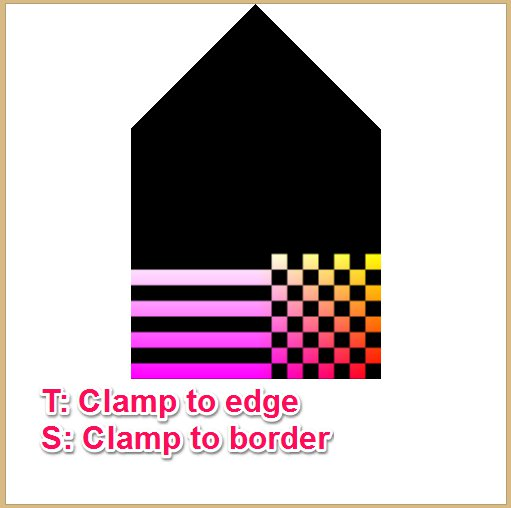
\includegraphics[width=0.35\textwidth]{figures/exercise_6_part_5_3}
	\end{center}
	\vspace{-4.5ex}\caption{Exercise 6 part 4-3 output}
	\label{fig:exercise_6_part_5_3} 
\end{figure}


\section{Part 5 and 6}
I succeded in making an animated texture assigning a transformation matrix of
rotation to a textureTrans uniform and multiplying texture coordinates with
that matrix. 
\begin{lstlisting}[language=cpp, caption={Texture animation - main.cpp}]
mat4 textureTrans = RotateZ(rotation);
glUniformMatrix4fv(textureTransUniform, 1, GL_TRUE, textureTrans);
\end{lstlisting}
\begin{lstlisting}[language=cpp, caption={Texture animation - tex-shader.vert}]
vTextureCoord = (textureTrans * vec4(textureCoord,0.0,1.0)).xy;
\end{lstlisting}
I obtained results which can be seen in the figure \ref{fig:exercise_6_part_6}
\begin{figure}[ht!]
	\begin{center}
		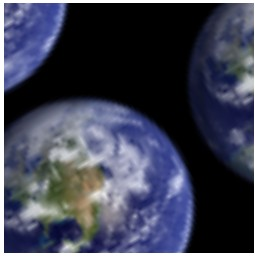
\includegraphics[width=.8\textwidth]{figures/exercise_6_part_6}
	\end{center}
	\vspace{-4.5ex}\caption{Exercise 6 part 5 and 6 output}
	\label{fig:exercise_6_part_6} 
\end{figure}